\section{Synchronisation in verteilen Systemen}
\subsection{Systemmodell}
% Events: senden, empfangen, internal
Dieser Abschnitt beschreibt ein vereinfachtes Modell eines verteilten Systems, welches als Grundlage für alle weiteren Ausführungen heran gezogen wird.
Der Einfachheit halber wird ein sehr grundlegendes Modell verwendet, welches jedoch ausreichend ist um die in dieser Arbeit geschilderten Zusammenhänge darzustellen, ohne Beschränkung der Allgemeinheit.

In unserem Modell besteht ein verteiltes System aus $n$ Prozesse die durch die Menge $P=\{p_1, p_2,\ldots, p_n\}$ beschrieben sind.
Die Prozesse können lediglich durch das Senden und Empfangen von Nachrichten kommunizieren.
Dabei wird angenommen, dass Nachrichten zuverlässig verschickt werden und somit in jedem Fall, nach einer gewissen Verzögerung, beim Empfänger ankommen.
Nachrichten müssen nicht zwangsläufig in der selben Reihenfolge ankommen in der sie gesendet wurden.
Dies ist dem Übertragungsweg geschuldet.

Ein Prozess $p_i$ besteht aus einer Sequenz von Ereignissen $E_i=\{e_i^1, e_i^2, \ldots\}$, welche eine totale Ordnung aufweisen.
Die Menge $E$ enthält alle Ereignisse die im kompletten System auftreten.
Diese Ordnung ergibt sich durch den Programmablauf des Prozesses und wird durch die Relation $\rightarrow$ beschrieben.
Löst ein Prozess $p_i$ zum Beispiel zuerst ein Ereignis $e_i^x$ aus und anschließend ein Zweites $e_i^y$, gilt $e_i^x \rightarrow e_i^y$. \fig{fig:genericEvents} zeigt eine exemplarische Kommunikation zwischen drei Prozessen und deren Ereignisse.

Jedes Ereignis ist atomar und stellt eine Zustandsänderung des dazugehörigen Prozesses dar.
Für die in dieser Arbeit beschriebenen Verfahren sind von besonderer Interesse die \qq{gesendet}- und \qq{empfangen}-Ereignisse.
Diese Ereignisse weisen Abhängigkeiten unter den Prozessen auf, welche die Notwendigkeit schafft die Prozesskommunikation zu synchronisieren.
Beiden Ereignisse können daher als Erweiterung der lokalen Programmordnung eines Prozesses auf das verteilte System betrachtet werden.

\begin{figure}[ht]
    \centering
    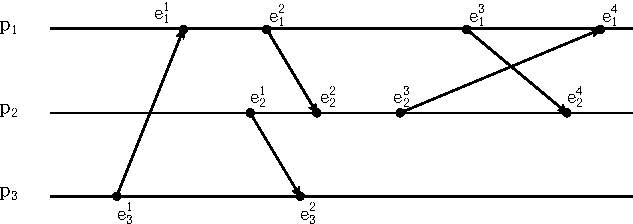
\includegraphics[width=12cm]{2_generic_events.pdf}
    \caption[Beispiel einer beliebigen Kommunikation]{TODO}
    \label{fig:genericEvents}
\end{figure}

Außerdem geht unser Modell davon aus, dass ein Prozess aus drei Schichten besteht.
Dies ist für die theoretische Definition unwesentlich, erleichtert aber die praktische Umsetzung und verbessert das Verständnis.
Die höchste Schicht ist die Anwendungsschicht, hier wird die Applikationslogik implementiert die durch das verteilte System abgebildet werden soll.
In der mittleren Schicht wird die Synchronisation der Kommunikation vorgenommen und kann somit für die Anwendungsschicht transparent  erfolgen.
Die unterste Schicht stellt die Netzwerkschicht dar, die Aufgabe dieser Schicht ist es die Nachrichten physikalisch zu übertragen.

\subsection{Kausalität und Ordnung}
\label{cap:ordnung}
% ungeordnet
% kausale Ordnung
% partielle kausale Ordnung
% totale Ordnung
Der Zusammenhang zwischen Ursache und Wirkung wird als Kausalität bezeichnet.
Es wird also die Abfolge von aufeinander bezogenen Ereignisse oder Zustände betrachtet.
Meist ist es nicht direkt ersichtlich ob Ereignisse kausal zusammenhängen, hierzu müssen die Gegebenheiten und Zusammenhänge der Ereignisse genau bekannt sein.
Dies ist nicht immer gegeben und auch nicht einfach entscheidbar. % TODO Beispiel wo es nicht einfach ist?
Daher wird im folgenden immer von potentieller Kausalität gesprochen.
Das bedeutet, dass nur Aussagen darüber gemacht werden ob ein Ereignis die Ursache für ein Anderes sein kann.

In einem einzelnen nicht nebenläufigen Prozess ist die potentielle Kausalität gegeben durch den Programmablauf.
Da die Instruktionen eines Programmes nacheinander ohne Vergabelungen ausgeführt werden und dabei jede Instruktion atomar ist, kann der aktuelle Zustand nur aus den davor ausgeführten Instruktionen bestimmt worden sein.
Hierbei kann eine Instruktion analog zu einem Ereignis verstanden werden.

Im Vergleich hierzu ist die Situation in einem verteilten System oder nebenläufigen Prozess deutlich komplexer.
Durch die Verteilung und Parallelität des Programmcodes ist die \qq{natürliche} Ordnung nicht mehr gegeben.
Innerhalb eines Prozesses ist die Ordnung weiterhin gegeben, da sich ein lokaler Prozess wie oben geschildert verhält.
Wird nun aber das Gesamtbild, also das ganze System betrachtet, sind die Eigenschaften von oben nicht mehr gegeben.
Das Wissen um die Kausalität der Ereignisse ist jedoch häufig notwendig um die Konsistenz des Systems zu wahren.

% TODO Konsitenz erklären vlt hier?

Der potentielle kausale Zusammenhang zwischen Ereignisse kann durch die Zeit festgestellt werden.
Ein Ereignis, welches zu einem späteren Zeitpunkt eingetreten ist, kann unmöglich die Ursache für ein vorhergehendes Ereignis sein.
Sind also die Zeitpunkte der Ereignisse bekannt, kann eine Aussage über die Kausalität getroffen werden.
Menschen haben ein intuitives Verständnis solcher Zusammenhänge.

Eine zeitliche Ordnung der Ereignisse ist somit die Grundlage für die Erkennung kausaler Zusammenhänge.
Ein Computer hat natürlich kein intuitives Verständnis von Zeit.
Daher müssen einige mathematische Definitionen festgelegt werden, welche die Grundlage für die Implementierung der zeitlichen Ordnungen dienen.

Damit eine Ordnung hergestellt werden kann, müssen die Ereignisse in Relation gesetzt werden können.
Eine Relation wurde bereits beschrieben, nämlich die \qq{Programmordnung} $\rightarrow$.
Lamport \cite{Lamport1978} definiert in seiner Arbeit die \qq{happend before}-Relation $\Rightarrow$ und stellt die kleinste Relation dar, die folgende Bedingungen erfüllt:
\begin{itemize}
    \item Wenn $e_i^x \rightarrow e_i^y$, dann $e_i^x \Rightarrow e_i^y$.
    \item Wenn $e_i^x$ ein Senden Ereignis ist und $e_j^y$ das Empfangen Ereignis der selben Nachricht darstellt, dann folgt $e_i^x \Rightarrow e_j^y$.
    \item Wenn $e_i^x \Rightarrow e_j^y$ und $e_j^y \Rightarrow e_k^z$, dann $e_i^x \Rightarrow e_k^z$.
\end{itemize}

Aus der ersten Bedingung ist ersichtlich, dass aus der strengeren Programmordnung direkt die \qq{happend before}-Relation für zwei lokale Ereignisse abgeleitet werden kann.
Die zweite Bedingung fordert, dass das Empfang Ereignis einer Nachricht nie vor dem Senden Ereignis eintreten kann.
Offensichtlich kann also eine Nachricht nicht empfangen werden, wenn sie noch nicht verschickt wurde.
Dieser Zusammenhang ist für Menschen zwar intuitiv ersichtlich kann nun aber auch für Computer korrekt formuliert werden.
Durch die dritte Bedingung ist die Transitivität der Relation gegeben.
Wurde ein Ereignis $z$ nach $y$ ausgelöst und $x$ vor $y$ gilt logischerweise, dass $x$ auch vor $z$ ausgelöst werden musste und somit $x\Rightarrow z$ gilt.

Ein Ereignis $e_j^y$ gilt als kausal abhängig von $e_i^x$ wenn $e_i^x \Rightarrow e_j^y$, da es nur ausgeführt werden kann wenn die Ausführung von $e_i^x$ bereits abgeschlossen ist.
Alternativ kann $e_i^x$ als Vorbedingung von $e_j^y$ betrachtet werden.

Zwei Ereignisse gelten als gleichzeitig aufgetreten wenn $e_i^x \centernot\Rightarrow e_j^y$ und $e_j^y \centernot\Rightarrow e_i^x$ gilt.
Dann können diese beiden Ereignisse parallel ausgeführt werden, da keines das jeweils Andere kausal beeinflussen kann.
Diese Nebenläufigkeit wird in Symbolen als $e_i^x \parallel e_j^y$ geschrieben.

Es ist offensichtlich, dass jede korrekte logische Uhr die \qq{happend before}-Relation einhalten muss.
Lamport folgert daraus die Uhrbedingung (engl. \qq{clock condition}) die von jeder korrekten logischen Uhr erfüllen muss:
\begin{equation*}
\forall e_i^x, e_j^y \in E \colon \text{wenn } e_i^x \Rightarrow e_j^y \text{ dann } C(e_i^x) < C(e_j^y)
\end{equation*}
%TODO In Worte fassen, was diese Bedinung aussagt
Aus dieser Uhrbedingung lassen sich zwei konkrete Bedingungen an den Uhren ableiten, welche sich direkt aus der Definition der $\Rightarrow$-Relation ergeben:
\begin{itemize}
    \item Wenn $e_i^x \rightarrow e_i^y$, dann $C(e_i^x) < C(e_i^y)$.
    \item Wenn $e_i^x$ ein Senden Ereignis ist und $e_j^y$ das Empfangen Ereignis der selben Nachricht darstellt, dann folgt $C(e_i^x) < C(e_i^y)$.
\end{itemize}

Die dritte Bedingung aus der Definition der \qq{happend before}-Relation muss hier nicht explizit wiederholt werden, da diese lediglich die Transitivität beschreibt und diese durch die $<$-Relation der Uhren gegeben ist.

Die eingeführten Regeln erlauben es nun die Zusammenhänge zwischen Ereignisse genauer zu betrachten.
Zustellungsregeln (engl. \qq{delivery rules}) definieren Einschränkungen an der Reihenfolge wie eingehende Nachrichten an den zu verarbeiteten Prozess verschickt werden dürfen.
Eine wichtige Regel ist die FIFO-Zustellung (\qq{First In First Out}) die besagt, dass ein Prozess $j$ Nachrichten in der Reihenfolge empfangen muss wie sie von $i$ aus gesendet wurden.
Dabei können Nachrichten von anderen Prozessen in beliebiger Reihenfolge versandt werden.
Es gilt somit
\begin{equation*}
    \text{wenn } e_i^s \rightarrow e_i^S \text{ dann } e_j^r \rightarrow e_j^R,
\end{equation*}
wobei $s$ und $S$ Sende-Ereignisse darstellen und $r/R$ die entsprechenden Empfang-Ereignisse sind.
In dieser Definition ist keine bestimmte Reihenfolge an Ereignisse von anderen Prozessen gefordert.

Eine weitere, im Vergleich zur FIFO-Zustellung strengere, Zustellungsregel ist die kausale Zustellung (engl. \qq{causal delivery}). Diese ist gegeben 
\begin{equation*}
    \text{wenn } e_i^s \Rightarrow e_k^S \text{ dann } e_j^r \rightarrow e_j^R.
\end{equation*}

Kausale Zustellung erweitert die FIFO-Zustellung um die Einschränkung, dass gesendete Nachrichten von verschiedenen Prozessen geordnet werden, sofern diese kausal nach der \qq{happend before}-Relation zusammenhängen.

Damit ein kausale Zustellung implementiert werden kann, muss die Uhr in der Lage sein Aussetzer in der Kommunikation zu erkennen.
Diese Eigenschaft wird Unterbrechungserkennung (engl. \qq{gap detection}) genannt.
Sie beschreibt den Umstand, dass ein Prozess in der Lage sein muss anhand zweier eingehender Nachrichten und deren Zeitstempel erkennen können muss, dass eine Nachricht existiert die in der Reihenfolge zwischen den beiden vorhanden Nachrichten gehört und bisher nicht empfangen wurde.
Formell gesprochen muss für zwei gegebenen Uhren $C_i(e_i^x) < C_j(e_j^y)$ entschieden werden, ob ein Ereignis $e_k^z$ mit $C_i(e_i^x)<C_k(e_k^z)<C_j(e_j^y)$ existiert \cite{babaoglu1993consistent}.

\subsection{Uhren}
In diesem Kapitel werden unterschiedliche Uhrtypen vorgestellt.
Generell wird zwischen physikalischen und logischen Uhren unterschieden \cite{Tanenbaum2007}.
Die im vorherigen Abschnitt beschrieben Zusammenhänge ermöglichen es logische Uhren formell zu definieren.
Bevor jedoch logische Uhren genauer beschrieben werden, wird zu erst auf physikalische Uhren eingegangen um den Unterschied zu logischen Uhren und deren Motivation zu verdeutlichen.

\subsubsection{Physikalische Uhren}
In der Regel besitzen heutige CPUs Schaltkreise die als Zeitgeber für die Uhrzeit verwendet werden.
Obwohl häufig als Uhr bezeichnet handelt es sich hierbei viel mehr um einen Zähler.
Ein im Prozessor integrierter Quarzkristall schwingt bei angelegter Spannung mit einer fest definierten Frequenz.
Mit dieser gegeben Frequenz kann nun ein Zähler pro Sekunde einmal inkrementiert werden und somit als Zeitgeber verwendet werden.

Bisher wurde die Darstellung eines Zeitpunktes weitestgehend ignoriert. Es liegt nahe, dass die für Menschen intuitive aufgeteilte Darstellung von Datum und Uhrzeit für Computer umständlich ist. Daher gibt es unterschiedliche Systeme, wie ein Zeitpunkt dargestellt werden kann.

Ein gängiges System um Zeitpunkte zu bestimmen ist die Unixzeit.
Dabei werden alle Sekunden seit dem 1. Januar 1970 um 00:00:00 Uhr UTC gezählt.
Ein Zeitpunkt kann daher einfach als Ganzzahl dargestellt werden.
Der große Vorteil dieses Systems liegt in seiner Einfachheit.
So kann mit einer Rechenoperation die Zeitdauer zwischen zwei Timestampes berechnen oder durch einen einfachen Vergleich festgestellt werden, welcher Timestamp weiter in der Vergangenheit liegt.

Wird nun jedem Ereignis in einem verteilten System ein Unix-Timestamp zugewiesen, kann theoretisch eine zeitliche Ordnung der Ereignisse über Prozessgrenze hinaus erreicht werden. Dies wird durch eine einfache Sortierung nach dem Zeitstempel erzielt.
Ein Problem dieser Herangehensweise ist die Auflösung des Zeitstempels. Treten mehrere Ereignisse innerhalb einer Sekunde auf, kann ihre Reihenfolge nicht am Timestamp festgestellt werden, da sich dieser logischerweise nur jede Sekunde ändert.

Hier ist die Unixzeit nicht mehr ausreichend und eine andere, genauere Darstellung muss gewählt werden.
Dabei steigt jedoch die Komplexität bei der Verarbeitung der Zeitstempel.
Zusätzlich ist nicht sofort klar, welche Darstellung als genau genug gilt.
Je kleiner der zeitliche Unterschied zwischen zwei Zeitstempeln desto genauer das System.
Hierbei muss ein Kompromiss zwischen Genauigkeit, Speicherbedarf und Verarbeitungsaufwand gefunden werden.

Ein weiteres Problem von physikalischen Uhren ist ihre Abweichung von der tatsächlichen Zeit.
So besitzt jeder Quartzkristall eine gewisse Schwankung in seiner Frequenz.
Dadurch driftet die Computeruhr immer weiter von der tatsächlichen Zeit ab.
Umgangssprachlich würde man sagen, die Uhr geht vor bzw. nach.
Dieses Abdriften lässt sich nur durch Verwendung von genaueren Uhren wie z.B. Atomuhren vermeiden.
Es ist jedoch unpraktikabel in jeden Computer eine Atomuhr zu installieren, daher muss die Uhr eines Computers mit einer anderen exakten Uhr regelmäßig synchronisiert werden.
In Netzwerken wird hierzu in der Regel das in der Einleitung erwähnte NTP Protokoll verwendet.

Für ein verteiltes System kann der absolute Fehler einer Uhr vernachlässigt werden, solang alle beteiligten Prozesse den selben Fehler haben und somit relativ innerhalb des Systems richtig sind.
Liegen zum Beispiel die Uhren aller Prozesse exakt 10 Sekunden in der Vergangenheit, kann die Reihenfolge der Ereignisse immer noch festgestellt werden. Weisen jedoch nur manche Prozesse einen Fehler auf, kann die Reihenfolge nicht mehr korrekt aus den Zeitstempel erschlossen werden.

Dieser Abweichung einzelner Uhren kann durch geeigneter Algorithmen entgegnet werden.
Ein solcher Algorithmus ist der Berkeley-Algorithmus. Dieser erfordert jedoch einen globalen Zeitgeber.
Es ist allgemein akzeptiert, dass eine globale physikalische Uhr für verteile System nicht tauglich ist. % TODO voll die Behauptung

\subsubsection{Lamport Uhren}
Leslie Lamport beschreibt in seinem Paper \cite{Lamport1978} von 1978, indem er gleichzeitig kausale Ordnung definiert, ein Verfahren um Prozesse durch logische Uhren zu synchronisieren.
Sein vorgeschlagener Algorithmus ist heute als Lamport Uhr bekannt und stellt eine simple Möglichkeit dar, partielle kausale Ordnung in einem verteilen System herzustellen.
Die Idee dahinter ist es, dass jeder Prozess einen eigenen Zähler, die Lamport Uhr, hält und bei Eintritt eines Ereignisses diese Zähler inkrementiert.
Sendet nun ein Prozess eine Nachricht, hängt er seinen aktuellen Zählerstand als Zeitstempel an die Nachricht an.
Empfängt nun ein anderer Prozess eine Nachricht kann er anhand des Zeitstempels der Nachricht und seiner lokalen Uhr den kausalen Zusammenhang erschließen.

Formall ist eine Lamportuhr durch eine Funktion definiert, welche einem Ereignis $e$ eine Nummer $C(e)$ zuweist.
Die Uhrbedingung aus Abschnitt~\ref{cap:ordnung} wird erfüllt indem jeder Prozess $i$ seine eigene Uhr $C_i$ hält und nach folgenden Regel aktualisiert:
\begin{itemize}
    \item Wenn $e_i^x$ kein Empfang-Ereignis ist, dann ist $C_i(e_i^x)=C_i(e_i^{x-1})+1$
    \item Ist $e_i^x$ ein Empfang-Ereignis der Nachricht $m$, dann ist $C_i(e_i^x)=\max\{C_i(e_i^{x-1}), C_j(e_j^y)  \} + 1$, wobei Prozess $j$ die Nachricht $m$ an $i$ geschickt hat und $C_j(e_j^y)$ der Uhrwert des Sende-Ereignis ist.
\end{itemize}

\begin{figure}[ht]
    \centering
    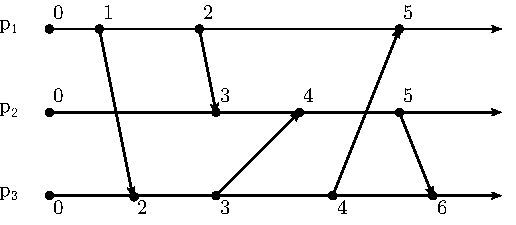
\includegraphics[width=0.80\textwidth]{LamportBeispiel.pdf}
    \caption[Exemplarische Kommunikation mit Lamport Uhr]{Kommunikation zwischen drei Prozessen unter Verwendung von Lamportuhren.}
    \label{fig:lamportBsp}
\end{figure}

% negativ Beispiel in Plausible Clocks Constant Size Logical Clocks for Distributed Systems
\subsubsection{Vektor Uhren}
\subsubsection{Interval Tree Uhren}